\textbf{\underline{\large{3.2: Definite Integrals and the Substitution Rule}}} \par

Now, it's time to revisit $u$-substitution within the context of definite integrals. Although the process is largely similar, there are some nuances that we must consider. \par

\begin{tcolorbox}[objective]
    \begin{center}
        OBJECTIVES \\[11pt]
    \end{center}
    Evaluate Definite Integrals Using the Fundamental Theorem of Calculus. \\
    Evaluate Definite Integrals Applying the Substitution Rule, When Appropriate. \\
    Use Proper Notation When Evaluating These Integrals
\end{tcolorbox} \vspace{11pt}

\begin{tcolorbox}[example]
    \textbf{Ex 3.2.1: } Evaluate $\int_0^2 t^2\sqrt{t^3 + 1} \, dx$.
\end{tcolorbox}
\begin{tcolorbox}[solution]
    \textbf{Sol 3.2.1: } Now, this problem may look just like a regular $u$-substitution problem that we did in the previous chapter. However, when we switch our integration variable to $u$, we also need to make sure to switch our definite integration boundaries to match. Let's see what that means in the solution below. \begin{align*}
        \int_0^2 t^2\sqrt{t^3 + 1} \, dt &= \dfrac{1}{3}\int_0^2 3t^2\sqrt{t^3 + 1} \, dt \\[5.5pt]
        \curvedarrow u = t^3 + 1 &\bargap \curvedarrow du = 3t^2 \, dt
    \end{align*}
    Here is where we have to be careful. We cannot simply rewrite our definite integral in terms of $u$, since our upper and lower boundaries are in terms of $t$! Therefore, we need to also find our new boundaries for the $u$ variables. Luckily, we can do this simply by plugging in our $t$ values into our equation for $u$. \begin{align*}
        u(0) = (0)^3 + 1 = 1 \bargap u(2) = (2)^3 + 1 = 9
    \end{align*}
    Now, we can continue integrating! (Note the boundary change in red.) \begin{align*}
        \dfrac{1}{3}\int_{\textcolor{red}{0}}^{\textcolor{red}{2}} 3t^2\sqrt{t^3 + 1} \, dt &= \dfrac{1}{3}\int_{\textcolor{red}{1}}^{\textcolor{red}{9}} \sqrt{u} \, du \\[5.5pt]
        & = \dfrac{1}{3}\left(\dfrac{2}{3}u^{\frac{3}{2}}\right) \eval_1^9 \\[5.5pt]
        & = \dfrac{2}{9}\left(9^{\frac{3}{2}} - 1^{\frac{3}{2}}\right) \\[5.5pt]
        & = \boxed{\dfrac{52}{9}}
    \end{align*}
\end{tcolorbox} \vspace{11pt}

\begin{tcolorbox}[example]
    \textbf{Ex 3.2.2: } Evaluate $\int_0^{\sqrt{\pi}} x\cos \left(x^2\right) \, dx$.
\end{tcolorbox}
\begin{tcolorbox}[solution]
    \textbf{Sol 3.2.2: } \begin{align*}
        \curvedarrow u = x^2 &\bargap \curvedarrow du = 2x \, dx \\[5.5pt]
        u(0) = (0)^2 = 0 &\bargap u\left(\sqrt{\pi}\right) = \left(\sqrt{\pi}\right)^2 = \pi \\[5.5pt]
        & = \dfrac{1}{2}\int_0^{\pi} \cos (u) \, du \\[5.5pt]
        & = \dfrac{1}{2}\sin (u) \eval_0^{\pi} \\[5.5pt]
        & = \boxed{0} 
    \end{align*}
\end{tcolorbox} \vspace{11pt}

\begin{tcolorbox}[example]
    \textbf{Ex 3.2.3: } Evaluate $\int_1^2 \dfrac{e^{\frac{1}{x}}}{x^2} \, dx$.
\end{tcolorbox}
\begin{tcolorbox}[solution]
    \textbf{Sol 3.2.3: } \begin{align*}
        \curvedarrow u = \dfrac{1}{x} &\bargap \curvedarrow du = -\dfrac{1}{x^2} \\[5.5pt]
        u(1) = \dfrac{1}{(1)} = 1 &\bargap u(2) = \dfrac{1}{(2)} = \dfrac{1}{2} \\[5.5pt]
        \int_1^2 \dfrac{e^{\frac{1}{x}}}{x^2} \, dx & = -\int_1^{\frac{1}{2}} e^u \, du \\[5.5pt]
        & = -e^u \eval_1^{\frac{1}{2}} \\[5.5pt]
        & = \boxed{-e^{\frac{1}{2}} + e}
    \end{align*}
\end{tcolorbox} \vspace{11pt}

\begin{tcolorbox}[example]
    \textbf{Ex 3.2.4: } Evaluate $\int_1^{\sqrt{13}} \dfrac{x}{x^2 + 3} \, dx$.
\end{tcolorbox}
\begin{tcolorbox}[solution]
    \textbf{Sol 3.2.4: } \begin{align*}
        \curvedarrow u = x^2 + 3 &\bargap \curvedarrow du = 2x \, dx \\[5.5pt]
        u(1) = (1)^2 + 3 = 4 &\bargap u\left(\sqrt{13}\right)^2 + 3 = 16 \\[5.5pt]
        \int_1^{\sqrt{13}} \dfrac{x}{x^2 + 3} \, dx &= \dfrac{1}{2}\int_1^{\sqrt{13}} \dfrac{2x}{x^2 + 3} \, dx \\[5.5pt]
        & = \dfrac{1}{2}\int_4^{16} \dfrac{1}{u} \, du \\[5.5pt]
        & = \dfrac{1}{2}\ln |u| \eval_4^{16} \\[5.5pt]
        & = \boxed{\dfrac{1}{2}\ln (16) - \dfrac{1}{2} \ln 4}
    \end{align*}
    \begin{tcolorbox}[interesting]
        Now, technically, $\dfrac{1}{2}\ln (16) - \dfrac{1}{2} \ln 4 \forcespace$ is the correct answer. However, when you are taking the multiple choice portion of the AP Calc BC exam, the expectation is that trivial logarithms should be simplified, so this answer may not appear as a choice. So, we must utilize our log rules: \begin{align*}
            \dfrac{1}{2}\ln (16) - \dfrac{1}{2} \ln 4 &= \dfrac{1}{2}\ln \left(\dfrac{16}{4}\right) \\[5.5pt]
            & = \dfrac{1}{2}\ln 4 \\[5.5pt]
            & = \ln 4^{\frac{1}{2}} \\[5.5pt]
            & = \boxed{\ln 2}
        \end{align*}
    \end{tcolorbox}
\end{tcolorbox}

\bigskip

\textbf{\large{The Average Value}}

One simple application of the definite integral is the Average Value Theorem. Recall that the average of a finite set of numbers is the total of the numbers divided by how many numbers we are averaging. Or, in technical terms: \begin{align*}
    \mathrm{avg} = \dfrac{\sum_{i = 1}^n x_i}{n}
\end{align*}

But, what does it mean to take the average value of a continuous function? Let's say you drive from home to school---what was your average velocity? What was the average temperature today? What was your average height for the first 15 years of your life? All these questions can be answered with the following formula: \par

\begin{center}
    \fbox{\fbox{\begin{minipage}{0.96\textwidth}
        \vspace{11pt}
        \begin{center}
            \textbf{The Average Value Formula}
        \end{center}
        \vspace{11pt}
        The average value of a function $f$ on a closed interval $[a, \, b]$ is defined by \begin{align*}
            f_{avg} = \dfrac{1}{b - a}\int_a^b f(x) \, dx \\
        \end{align*}
    \end{minipage}}}
\end{center}

If we look at this formula in the context of the Fundamental Theorem of Calculus, it will start to make a little more sense. \begin{align*}
    \int_a^b f(x) \, dx &= F(b) - F(a) \\[5.5pt]
    \dfrac{1}{b - a}\int_a^b f(x) \, dx &= \dfrac{1}{b - a}(F(b) - F(a)) \\[5.5pt]
    & = \dfrac{F(b) - F(a)}{b - a}
\end{align*}

Notice that this is just the average slope for $F(x)$ on $x \in [a, \, b]$. Since the derivative $F'(x)$ gives the instantaneous rate of change of $F(x)$, the average slope of $F(x)$ is the same as average value of $F'(x)$. But, since the definition in the Fundamental Theorem of Calculus says that $F'(x) = f(x)$, this is actually just the average value of $f(x)$. \par

\begin{tcolorbox}[example]
    \textbf{Ex 3.2.5: } Find the average value of $f(x) = x^2 + 1$ on $[0, \, 5]$.
\end{tcolorbox}
\begin{tcolorbox}[solution]
    \textbf{Sol 3.2.5: } We first start with our formula: \begin{align*}
        f_{avg} = \dfrac{1}{b - a}\int_a^b f(x) \, dx
    \end{align*}
    Then, we can substitute in the function and the interval. \begin{align*}
        f_{avg} = \dfrac{1}{5 - 0}\int_0^5 \left(x^2 + 1\right) \, dx
    \end{align*}
    Using either \fbox{\texttt{MATH}} \fbox{\texttt{9}} on our TI-84 or integrating analytically gives us $f_{avg} = \boxed{\dfrac{28}{3}}$.
\end{tcolorbox} \vspace{11pt}

\begin{tcolorbox}[example]
    \textbf{Ex 3.2.6: } Find the average value of $h(\theta) = \sec (\theta)\tan (\theta)$ on $\left[0, \, \dfrac{\pi}{4}\right]$.
\end{tcolorbox}
\begin{tcolorbox}[solution]
    \textbf{Sol 3.2.6: } \begin{align*}
        h_{avg} &= \dfrac{1}{b - a}\int_a^b h(\theta) \, d\theta \\[5.5pt]
        & = \dfrac{1}{\frac{\pi}{4} - 0}\int_0^{\frac{\pi}{4}} \sec (\theta)\tan (\theta) d\theta \\[5.5pt]
        & = \boxed{\dfrac{4}{\pi}\left(\sqrt{2} - 1\right) \approx 0.524}
    \end{align*}
\end{tcolorbox}

\newpage

\textbf{\large{3.2 Free Response Homework}} \par

\twoquestion{1. $\int_0^1 x^2\left(1 + 2x^3\right)^5 \, dx$}{2. $\int_0^1 x^3\left(x^4 + 5\right)^3 \, dx$} \\[11pt]
\twoquestion{3. $\int_{-1}^1 x\sqrt{4 - x^2} \, dx$}{4. $\int_1^2 \dfrac{x^2}{\sqrt[3]{9 - x^3}} \, dx$} \\[11pt]
\twoquestion{5. $\int_0^3 \dfrac{10t + 15}{\sqrt[4]{t^2 + 3t + 1}} \, dt$}{6. $\int_1^2 \dfrac{x + 1}{\sqrt{x^2 + 2x + 4}} \, dx$} \\[11pt]
\twoquestion{7. $\int_1^3 \dfrac{5t}{t^2 + 1} \, dt$}{8. $\int_{-1}^2 \dfrac{1}{2x + 5} \, dx$} \\[11pt]
\twoquestion{9. $\int_{\sqrt{3}}^2 ye^{y^2 - 3} \, dy$}{10. $\int_0^1 \dfrac{v^2}{8 - v^3} \, dv$} \\[11pt]
\twoquestion{11. $\int_3^{e^2 + 2} \dfrac{1}{x - 2} \, dx$}{12. $\int_0^{\frac{\pi}{3}} \dfrac{\sin (\theta)}{\cos^2 (\theta)} d\theta$} \\[11pt]
\twoquestion{13. $\int_e^{e^4} \dfrac{1}{x\sqrt{\ln x}} \, dx$}{14. $\int_0^{\pi} \sec^2 \left(\dfrac{t}{4}\right) \, dt$} \\[11pt]
\twoquestion{15. $\int_0^{\pi} \dfrac{\sin (x)}{2 - \cos (x)} \, dx$}{16. $\int_2^4 \dfrac{1}{x\ln x} \, dx$} \\[11pt]
\twoquestion{17. $\int_0^{\ln 2} \dfrac{e^x}{1 + e^{2x}} \, dx$}{18. $\int_{\frac{\pi}{6}}^{\frac{\pi}{2}} \cos^5 (x)\sin (x) \, dx$} \\[11pt]
\twoquestion{19. $\int_0^{\frac{\pi}{8}} \sec^2 (2x) \, dx$}{20. $\int_{e^{\frac{\pi}{4}}}^{e^{\frac{\pi}{2}}} \dfrac{\csc^2 (\ln y)}{y} \, dy$} \\[11pt]
\twoquestion{21. $\int_0^{\pi} \dfrac{\cos (x)}{2 + \sin (x)} \, dx$}{22. $\int_0^{\pi} \dfrac{\sin (y)}{2 + \cos (y)} \, dy$} \\[11pt]
\twoquestion{23. $\int_0^{\sqrt{\frac{\pi}{4}}} m\sec \left(m^2\right)\tan \left(m^2\right) \, dm$}{24. $\int_0^{\frac{\pi}{4}} \sec^2 (x)\tan^3 (x) \, dx$} \\[11pt]
\twoquestion{25. $\int_{\frac{\pi}{2}}^{\pi} \cos^9 (x)\sin (x) \, dx$}{26. $\int_0^{\pi} \cos^6 \left(\dfrac{x}{2}\right)\sin \left(\dfrac{x}{2}\right) \, dx$} \\[11pt]
\twoquestion{27. $\int_{\pi}^{2\pi} \cos \left(\dfrac{1}{2}\theta\right) \, d\theta$}{28. $\int_2^{e^3 + 1} \dfrac{(\ln (x - 1))^4}{x - 1} \, dx$} \\[11pt]
\twoquestion{29. $\int_0^{e^2 - 1} \dfrac{1}{x + 1} \, dx$}{30. $\int_5^{e^3 + 4} \dfrac{1}{x - 4} \, dx$} \\[11pt]

Find the average value of each of the following functions over the given interval. \par

\twoquestion{31. $F(x) = (x - 3)^2$ on $x \in [3, \, 7]$}{32. $H(x) = \sqrt{x}$ on $x \in [0, \, 3]$} \\[11pt]
\twoquestion{33. $F(x) = \sec^2 (x)$ on $x \in \left[0, \, \dfrac{\pi}{4}\right]$}{34. $F(x) = \dfrac{1}{x}$ on $x \in [1 \, 3]$} \\[11pt]
\twoquestion{35. $f(t) = t^2 - \sqrt{t} + 5$ on $t \in [1, \, 4]$}{36. $f(t) = t^2 - \sqrt{t} + 5$ on $t \in [4, \, 9]$} \\[11pt]
\twoquestion{37. $f(x) = \cos (x)\sin^4 (x)$ on $x \in [0, \, \pi]$}{38. $g(x) = xe^{-x^2}$ on $x \in [1, \, 5]$} \\[11pt]
\twoquestion{39. $G(x) = \dfrac{x}{\left(1 + x^2\right)^3}$ on $x \in [0, \, 2]$}{40. $h(x) = \dfrac{x}{\left(1 + x^2\right)^2}$ on $x \in [0, \, 4]$} \\[11pt]
\onequestion{41. If a cookie taken out of a $450^{\circ} \si{F}$ oven cools in a $60^{\circ} \si{F}$ room, then according to Newton's Law of Cooling, the temperature of the cookie $t$ minutes after it has been taken out of the oven is given by \begin{align*}
    T(t) = 60 + 390e^{-0.205t}.
\end{align*}
What is the average value of the cookie's temperature during its first 10 minutes out of the oven?} \\[11pt]
\onequestion{42. We know as the seasons change so do the length of the days. Suppose the length of the day varies sinusoidally with time by the equation \begin{align*}
    L(t) = 10 - 3\cos \left(\dfrac{\pi t}{182}\right),
\end{align*}
where $t$ is the number of days after the winter solstice (December 22, 2007). What was the average day length from January 1, 2008 to March 31, 2008?} \\[11pt]
\onequestion{43. During one summer in the Sunset, the temperature is modeled by the function \begin{align*}
    T(t) = 50 + 15\sin \left(\dfrac{\pi}{12}t\right),
\end{align*}
where $T$ is measured in $\mathrm{F}^{\circ}$ and $t$ is measured in hours after 7 a.m. What is the average temperature in the Sunset during the six-hour chemistry class that runs from 9 a.m. to 3 p.m.?} \\[11pt]

\textbf{\large{3.2 Multiple Choice Homework}} \par

\begin{questions}
    \question $\int_1^4 \dfrac{1}{\left(1 + \sqrt{x}\right)^2\sqrt{x}} \, dx$ \\

    \begin{oneparchoices}
        \choice $\dfrac{6}{5}$
        \choice $\dfrac{1}{3}$
        \choice $\dfrac{2}{3}$
        \choice $\dfrac{4}{9}$
        \choice $\dfrac{3}{2}$
    \end{oneparchoices} \par \horizontalline

    \question If $\int_1^4 h(x) \, dx = 6$, then $\int_1^4 h(5 - x) \, dx = $ \\

    \begin{oneparchoices}
        \choice $-6$
        \choice $-1$
        \choice $0$
        \choice $3$
        \choice $6$
    \end{oneparchoices} \par \horizontalline

    \question $\int_e^{e^2} \dfrac{1}{x \ln x} \, dx = $ \\

    \begin{oneparchoices}
        \choice $\ln (\ln 2)$
        \choice $\dfrac{2}{e^2}$
        \choice $\ln 2$
        \choice $\dfrac{1 - 2e}{2e^2}$
        \choice $DNE$
    \end{oneparchoices} \par \horizontalline

    \question Determine the average value of $y = e^{6x}$ on $x \in [0, \, 4]$. \\

    \begin{oneparchoices}
        \choice $\dfrac{e^{24} - 1}{4}$
        \choice $\dfrac{e^{24} - 1}{6}$
        \choice $\dfrac{e^{24}}{24}$
        \choice $\dfrac{e^{24}}{6}$
        \choice $\dfrac{e^{24} - 1}{24}$
    \end{oneparchoices} \par \horizontalline

    \question Determine the average value of $g(x) = (2x + 3)^2$ on $x \in [-3, \, -1]$. \\

    \begin{oneparchoices}
        \choice $\dfrac{7}{3}$
        \choice $-4$
        \choice $5$
        \choice $\dfrac{14}{3}$
        \choice $3$
    \end{oneparchoices} \par \horizontalline

    \question Determine the average value of $g(x) = e^{7x}$ on $x \in [0, \, 4]$. \\

    \begin{oneparchoices}
        \choice $\dfrac{1}{14}e^{14}$
        \choice $\dfrac{1}{7}\left(e^{14} - 1\right)$
        \choice $\dfrac{1}{14}\left(e^{14} - 1\right)$
        \choice $\dfrac{1}{2}\left(e^{14} - 1\right)$
        \choice $\dfrac{1}{7}e^{14}$
    \end{oneparchoices} \par \horizontalline

    \question If the function $y = x^3$ has an average value of $9$ on $x \in [0 , \, k]$, then $k = $. \\

    \begin{oneparchoices}
        \choice $3$
        \choice $\sqrt{3}$
        \choice $\sqrt[3]{18}$
        \choice $\sqrt[4]{36}$
        \choice $\sqrt[3]{36}$
    \end{oneparchoices} \par \horizontalline

    \question Find the average rate of change of $y = x^2 + 5x + 14$ on $x \in [-1 \, 2]$ \\
    
    \begin{oneparchoices}
        \choice $3$
        \choice $6$
        \choice $9$
        \choice $\dfrac{65}{6}$
        \choice $18$
    \end{oneparchoices} \par \horizontalline

    \question If the average of the function $f(x) = |x - a|$ on $[-1 \, 1]$ is $\dfrac{5}{4}$, what is/are the values of $a$? \\

    \begin{oneparchoices}
        \choice $\pm 1$
        \choice $\pm \dfrac{1}{2}$
        \choice $\pm \dfrac{1}{4}$
        \choice $0$
        \choice None of these
    \end{oneparchoices} \par \horizontalline

    \question What is the average rate of change of the function $f(x) = x^4 - 5x$ on the closed interval $[0, \, 3]$? \\

    \begin{oneparchoices}
        \choice $8.5$
        \choice $8.7$
        \choice $22$
        \choice $23$
        \choice $66$
    \end{oneparchoices} \par \horizontalline

    \question Determine the average value of $y = e^x\cos (x)$ on $x \in \left[0, \, \dfrac{\pi}{2}\right]$ \\

    \begin{oneparchoices}
        \choice $0$
        \choice $1.213$
        \choice $1.905$
        \choice $2.425$
        \choice $3.810$
    \end{oneparchoices} \par \horizontalline

    \question The graphs of five functions are shown below. Which function has a nonzero average value over the closed interval $x = [-\pi, \, \pi]$. \\

    \begin{oneparchoices}
        \choice 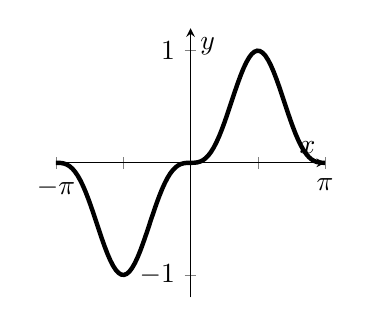
\begin{tikzpicture}
            \begin{axis}[
                axis lines = middle,
                xlabel = $x$,
                ylabel = $y$,
                domain = -pi:pi,
                samples = 100,
                width=5cm,
                height=5cm,
                xtick = {-3.14, -1.57, 0, 1.57, 3.14},
                xticklabels = {$-\pi$, , $0$, , $\pi$},
                ymin = -1.2, ymax = 1.2,
            ]
              \addplot[ultra thick] {(sin(deg(x)))^3};
            \end{axis}
        \end{tikzpicture}
        \choice 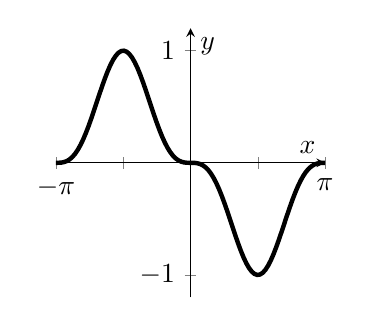
\begin{tikzpicture}
            \begin{axis}[
                axis lines = middle,
                xlabel = $x$,
                ylabel = $y$,
                domain = -pi:pi,
                samples = 100,
                width=5cm,
                height=5cm,
                xtick = {-3.14, -1.57, 0, 1.57, 3.14},
                xticklabels = {$-\pi$, , $0$, , $\pi$},
                ymin = -1.2, ymax = 1.2,
            ]
              \addplot[ultra thick] {-(sin(deg(x)))^3};
            \end{axis}
        \end{tikzpicture}
        \choice 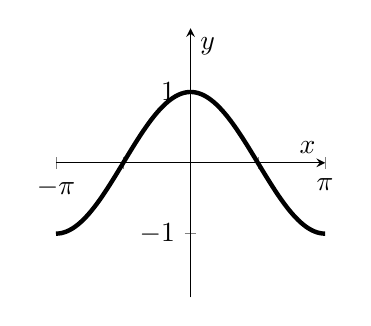
\begin{tikzpicture}
            \begin{axis}[
                axis lines = middle,
                xlabel = $x$,
                ylabel = $y$,
                domain = -pi:pi,
                samples = 100,
                width=5cm,
                height=5cm,
                xtick = {-3.14, -1.57, 0, 1.57, 3.14},
                xticklabels = {$-\pi$, , $0$, , $\pi$},
                ymin = -1.9, ymax = 1.9,
            ]
              \addplot[ultra thick] {cos(deg(x))};
            \end{axis}
        \end{tikzpicture} \\[22pt]
        \makebox[0.2\textwidth] \choice 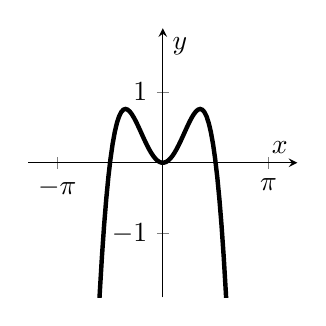
\begin{tikzpicture}
            \begin{axis}[
                axis lines = middle,
                xlabel = $x$,
                ylabel = $y$,
                domain = -pi:pi,
                samples = 100,
                width=5cm,
                height=5cm,
                xmin = -4, xmax = 4,
                xtick = {-3.14, -1.57, 0, 1.57, 3.14},
                xticklabels = {$-\pi$, , $0$, , $\pi$},
                ymin = -1.9, ymax = 1.9,
            ]
              \addplot[ultra thick] {-1/2 * x^4 + (3.14)^2/8 * x^2};
            \end{axis}
        \end{tikzpicture}
        \makebox[0.15\textwidth] \choice 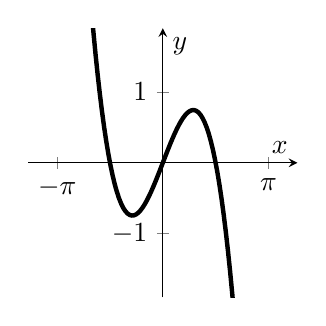
\begin{tikzpicture}
            \begin{axis}[
                axis lines = middle,
                xlabel = $x$,
                ylabel = $y$,
                domain = -pi:pi,
                samples = 100,
                width=5cm,
                height=5cm,
                xmin = -4, xmax = 4,
                xtick = {-3.14, -1.57, 0, 1.57, 3.14},
                xticklabels = {$-\pi$, , $0$, , $\pi$},
                ymin = -1.9, ymax = 1.9,
            ]
              \addplot[ultra thick] {-1/2 * x^3 + (3.14)^2/8 * x};
            \end{axis}
        \end{tikzpicture}
    \end{oneparchoices} \par \horizontalline
\end{questions}